\documentclass[25pt, a0paper, portrait]{tikzposter}
\usepackage[T1]{fontenc}
\renewcommand*\familydefault{\sfdefault}
\usepackage{sfmath}
\usepackage{amsmath}
\usepackage{lipsum}
\usepackage[compress]{cite}

\newcommand{\CORE}{The CORE collaboration}
\newcommand{\PLANCK}{The Planck collaboration}
\newcommand{\prd}{PRD}
\newcommand{\prr}{PRR}
\newcommand{\mnras}{MNRAS}
\newcommand{\jcap}{JCAP}
\newcommand{\jmap}{JMAP}
\newcommand{\joss}{JOSS}
\newcommand{\pasa}{PASA}
\newcommand{\aap}{A\&A}
\newcommand{\prl}{PRL}
\newcommand{\arxiv}{arXiv}



\makeatletter
\renewcommand\TP@maketitle{%
    \centering
    \vspace{-40pt}
    
\includegraphics[height=0.09\textwidth]{reach.png}\hfill
    \begin{minipage}[b]{0.7\linewidth}
        \centering
        \color{titlefgcolor}
        {\Huge \sc \@title \par}
        \vspace*{1em}
        {\huge \@author \par}
        \vspace*{1em}
        {\LARGE \@institute}
    \end{minipage}%
    \hfill
\includegraphics[height=0.09\textwidth]{cambridge-cropped.pdf}
}
\makeatother

\title{Poster: a template for a scientific poster in \LaTeX}
\author{Samuel Alan Kossoff Leeney <sakl2@cam.ac.uk>}
\institute{Kavli Institute for Cosmology $\cdot$ Cavendish Laboratory $\cdot$  University of Cambridge}
%\usetheme{Default}
%\usetheme{Rays}
%\usetheme{Basic}
%\usetheme{Simple}
\usetheme{Envelope}
%\usetheme{Wave}
%\usetheme{Board}
%\usetheme{Autumn}
%\usetheme{Desert}

\tikzposterlatexaffectionproofoff{}

\let\oldbibliography\thebibliography
\renewcommand{\thebibliography}[1]{\oldbibliography{#1}
\setlength{\itemsep}{-5pt}} %Reducing spacing in the bibliography.

\pdfinclusioncopyfonts=1 % Fix fonts on non-linux machines

\usepackage{xcolor}
\definecolor{C0}{HTML}{1f77b4}
\definecolor{C1}{HTML}{ff7f0e}
\definecolor{C2}{HTML}{2ca02c}
\definecolor{C3}{HTML}{d62728}
\definecolor{C4}{HTML}{9467bd}
\definecolor{C5}{HTML}{8c564b}
\definecolor{C6}{HTML}{e377c2}
\definecolor{C7}{HTML}{7f7f7f}
\definecolor{C8}{HTML}{bcbd22}
\definecolor{C9}{HTML}{17becf}
\newcommand\C[2][1]{\textcolor{C#1}{#2}}


%\usecolorstyle[colorOne=blue, colorTwo=gray, colorThree=green]{Default}
%\usecolorpalette{BlueGrayOrange}
%\usecolorstyle[colorOne=blue]{mystyle}
%\colorlet{backgroundcolor}{C1}

%% Background Colors
\colorlet{backgroundcolor}{C0!50!white}
\colorlet{framecolor}{black}
%% Title Colors
\colorlet{titlefgcolor}{white}
\colorlet{titlebgcolor}{C0}
%% Block Colors
\colorlet{blocktitlebgcolor}{C0}
\colorlet{blocktitlefgcolor}{white}
\colorlet{blockbodybgcolor}{white}
\colorlet{blockbodyfgcolor}{black}
%% Innerblock Colors
\colorlet{innerblocktitlebgcolor}{C1}
\colorlet{innerblocktitlefgcolor}{black}
\colorlet{innerblockbodybgcolor}{C1!10!white}
%\colorlet{innerblockbodyfgcolor{black}
%% Note colors
\colorlet{notefgcolor}{black}
\colorlet{notebgcolor}{C2!50!white}
\colorlet{notefrcolor}{C2}

\usepackage[hidelinks]{hyperref}
\hypersetup{
    colorlinks,
    linkcolor={C3!50!black},
    citecolor={C0!50!black},
    urlcolor={C0!80!black}
}

\begin{document}
\maketitle

    \block{}{%
        \centering
        
\includegraphics[height=0.09\textwidth]{kicc}
        \hspace{20pt}
        \begin{minipage}[b]{0.73\textwidth}
            \lipsum[1]
        \end{minipage}%
        \hspace{20pt}
        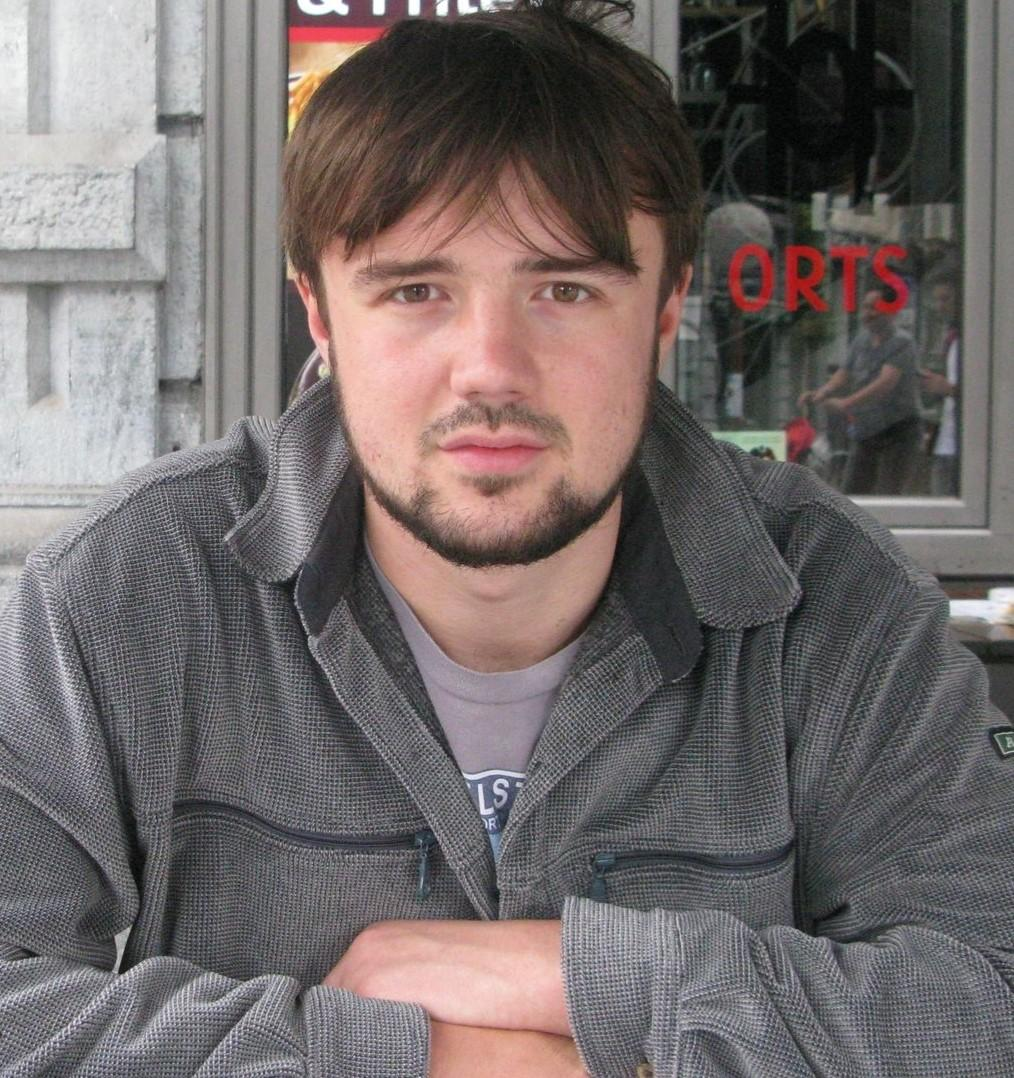
\includegraphics[height=0.09\textwidth]{avatar.jpg}

    }
\begin{columns}
    \column{0.5}

    \block{The first text box}{%
        \begin{tikzfigure}[The first figure caption]
        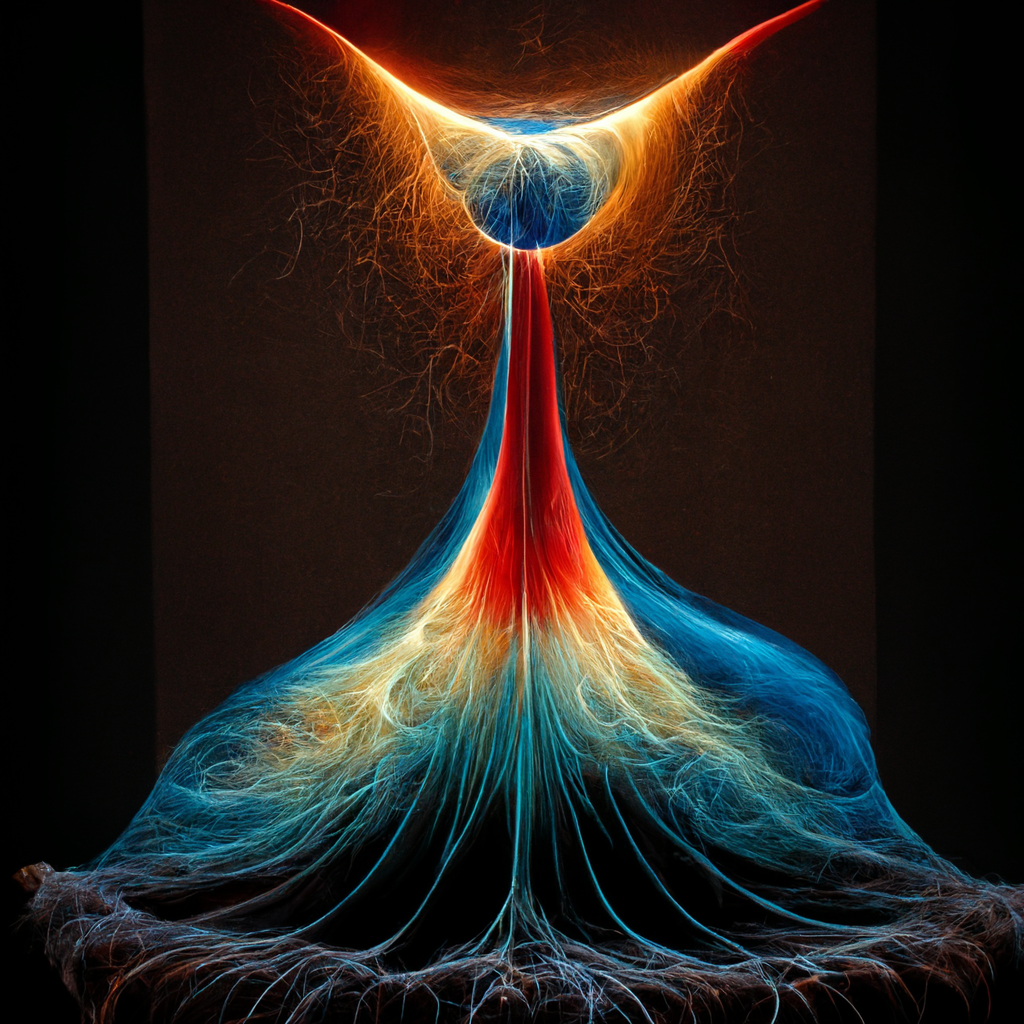
\includegraphics[height=0.13\textwidth]{image_1}
        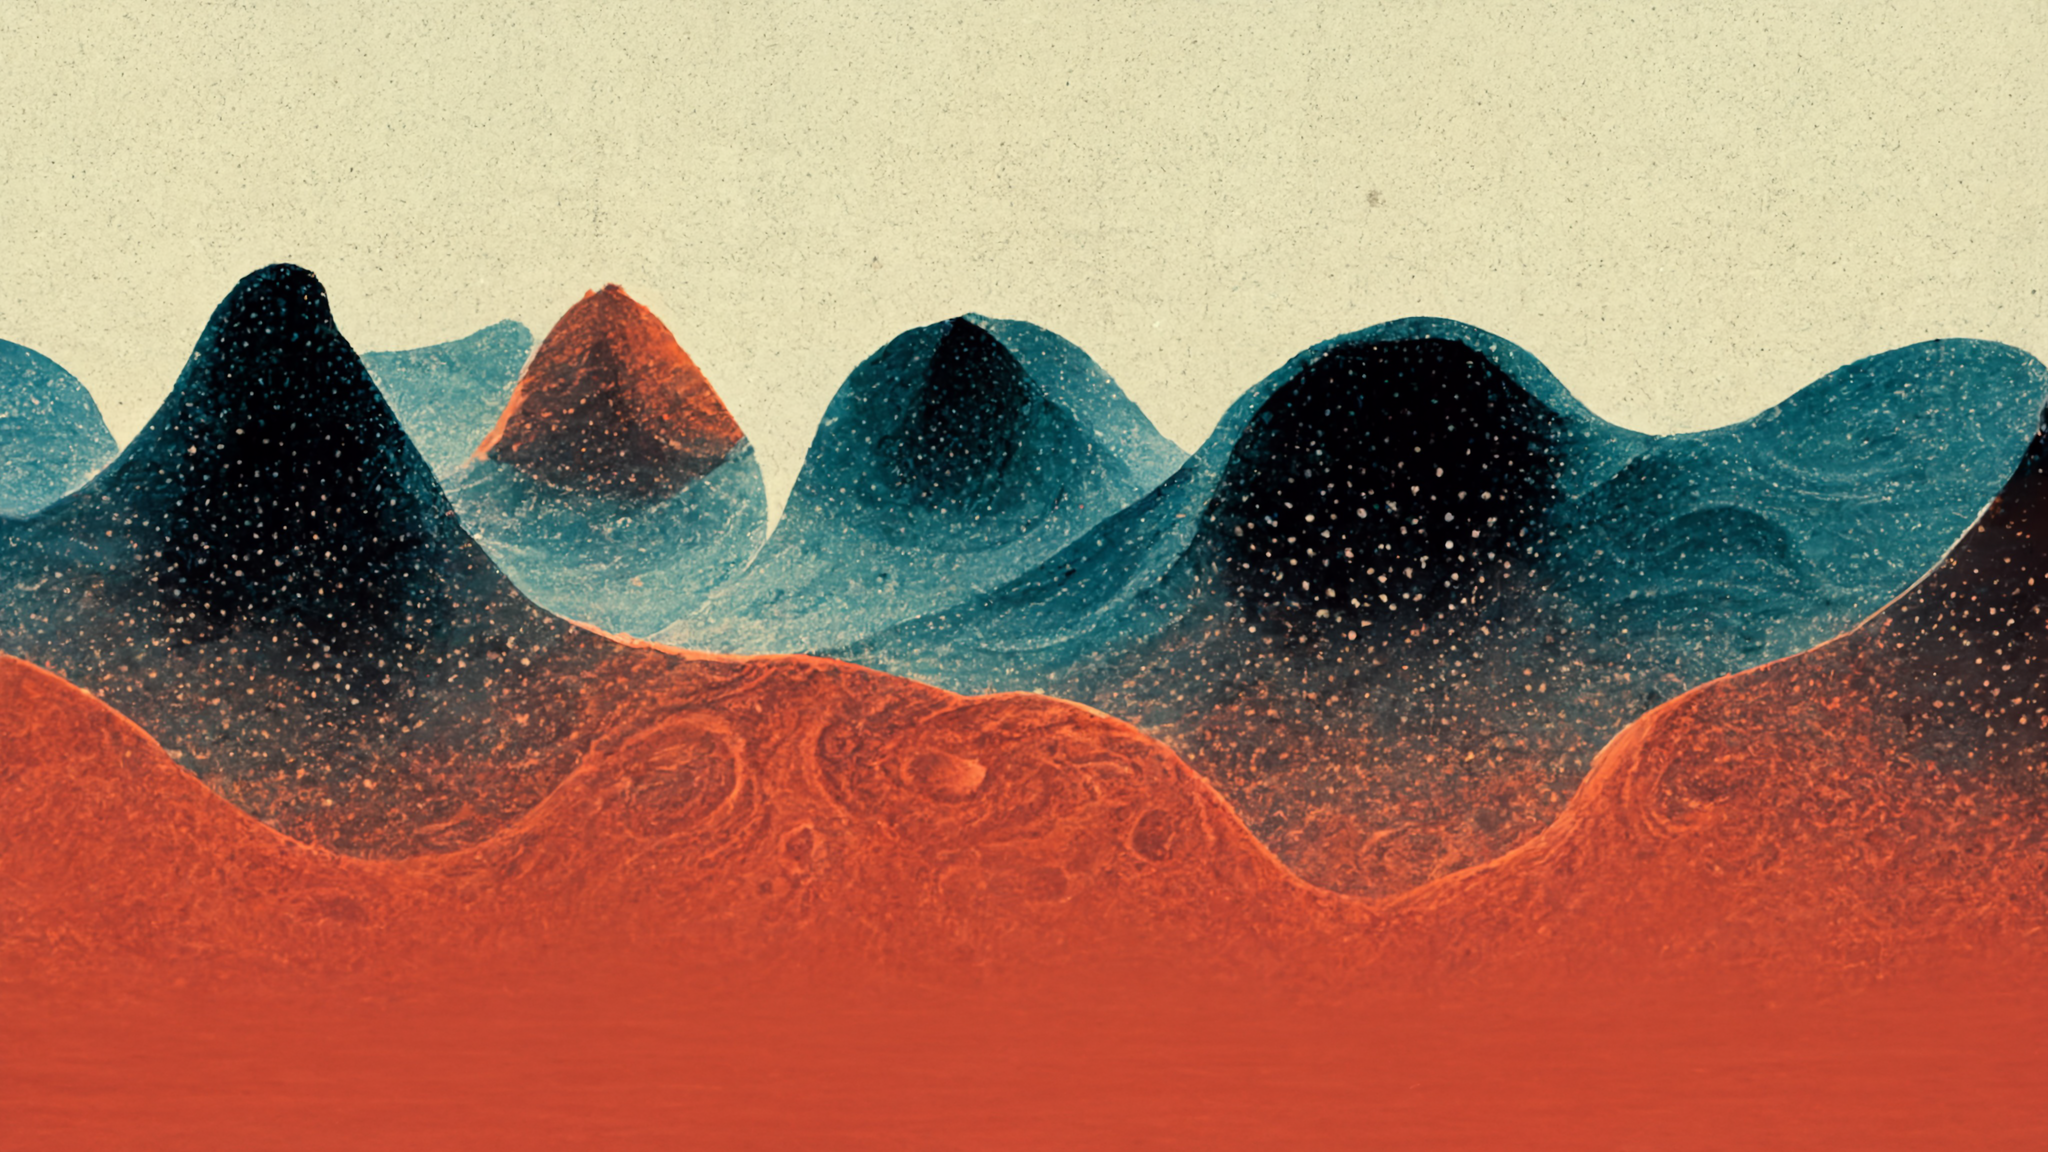
\includegraphics[height=0.13\textwidth]{image_5}
        \end{tikzfigure}
        \vspace{0.5em}
        \LaTeX is a high-quality typesetting system, it is excellent at mathematics, such as the equation of a circle $x^2 + y^2 = r^2$.
        \begin{center}
            \begin{tabular}{|ll|}
                \hline
                $A$: & The first letter of the roman alphabet. \\
                $\Omega$: & The last letter of the greek alphabet. \\
                \hline
            \end{tabular}
        \end{center}
        \vspace{0.5em}

        Here is Bayes theorem:
        \begin{equation}
            P(A|B) = \frac{P(B|A)P(A)}{P(B)}
            \nonumber
        \end{equation}
    }

    \block{Minipages}{%


        \begin{minipage}[]{0.2\textwidth}
            \centering
            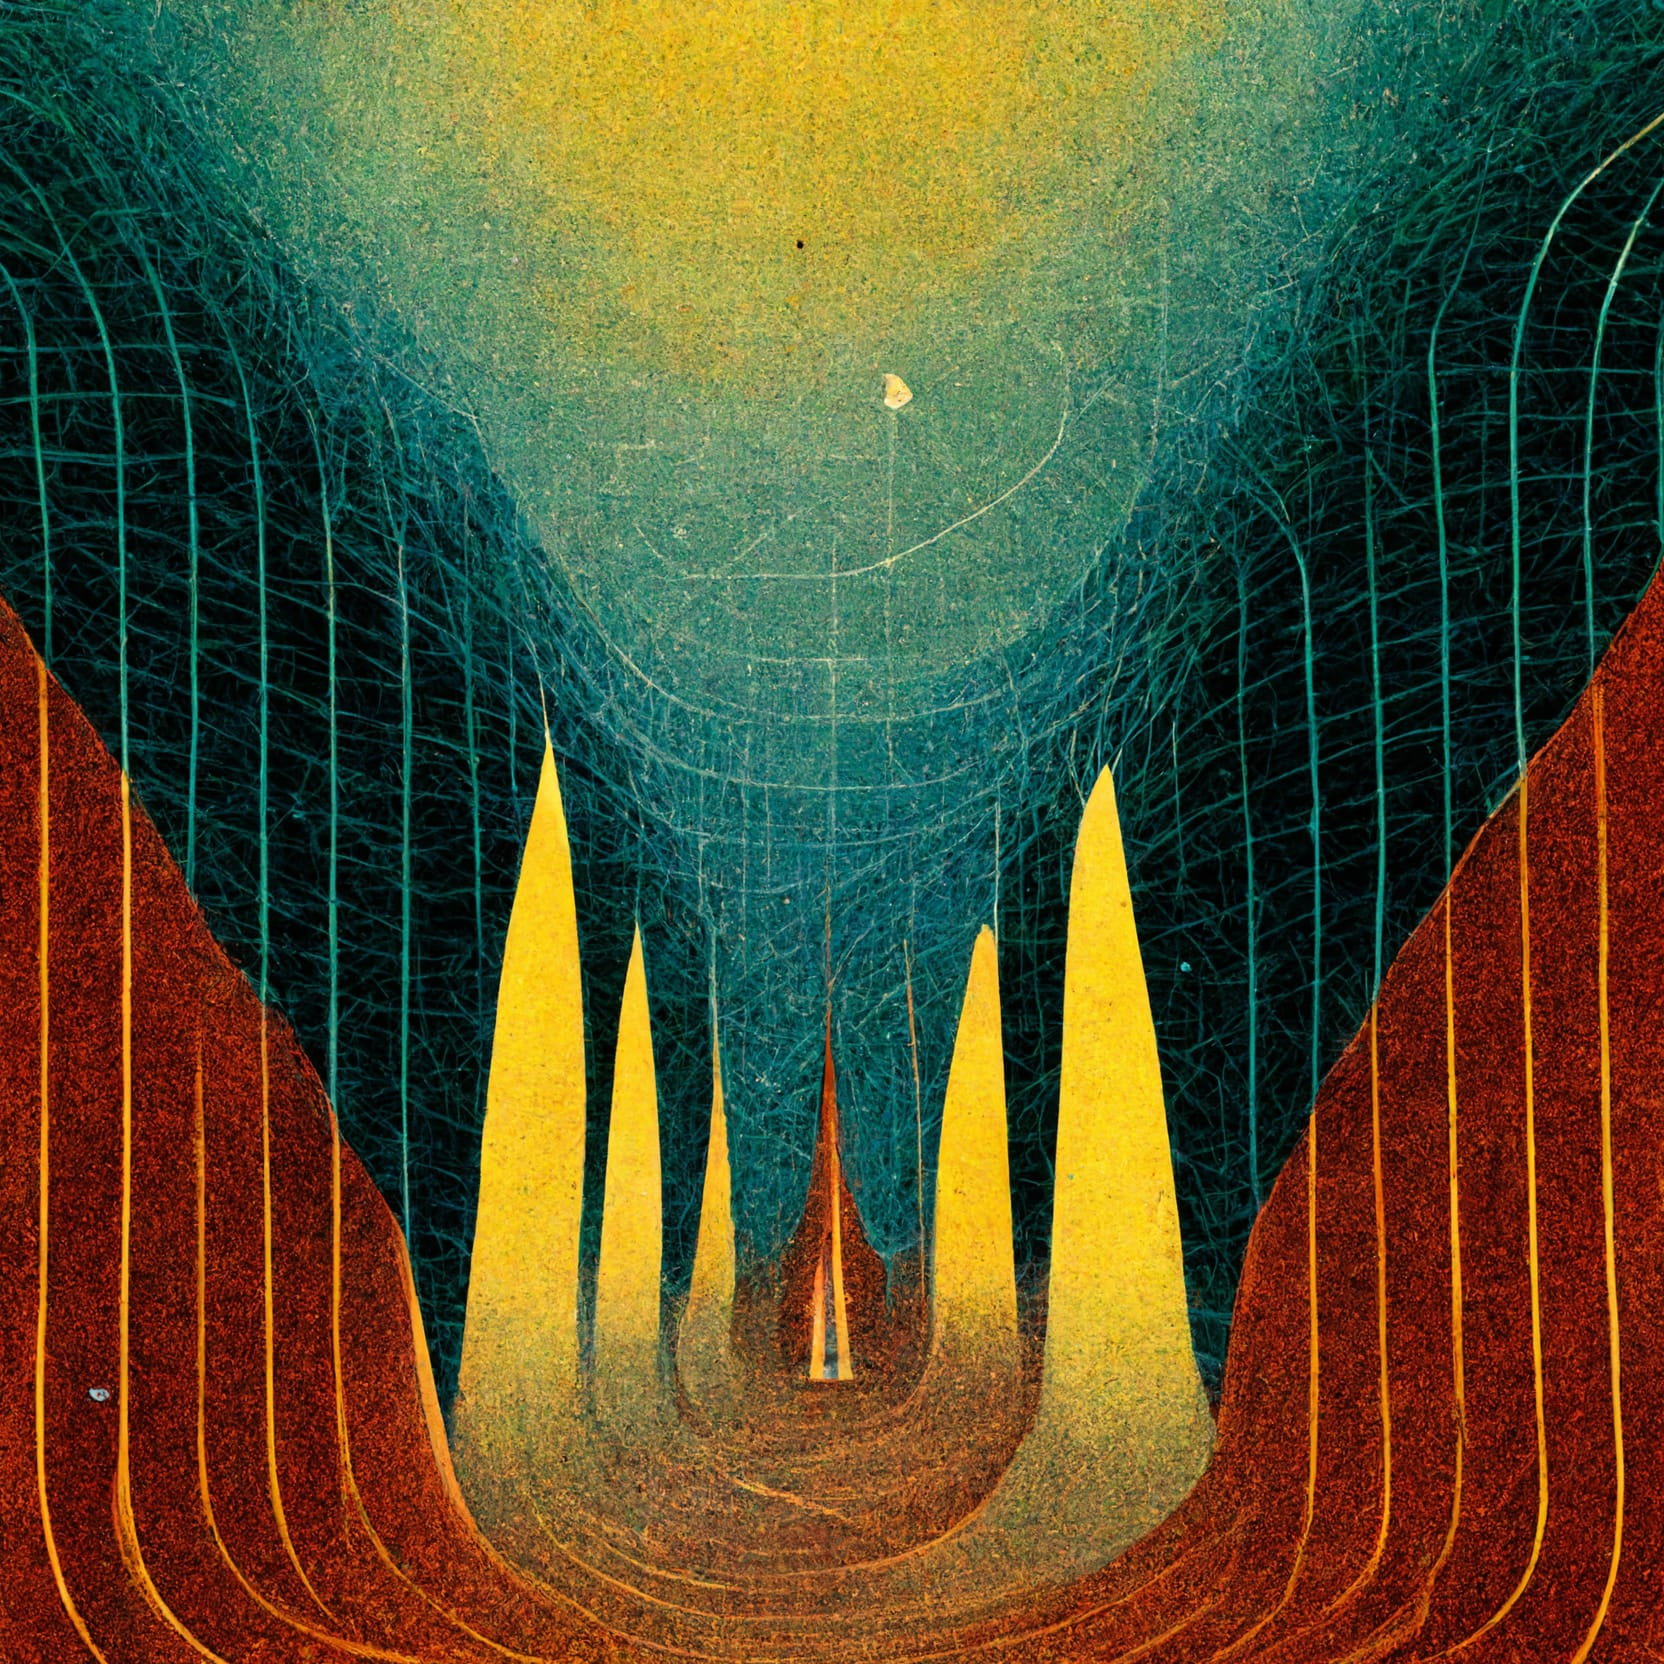
\includegraphics[width=\textwidth]{image_9}
        \end{minipage}\hfill
        \begin{minipage}[]{0.2\textwidth}
            Minipages can be useful for placing figures side-by-side. They can also be used to place text side-by-side with figures. Here is an example of a minipage with a figure on the left and text on the right.\\

            Here is Bayes theorem again
            \begin{equation}
                P(A|B) = \frac{P(B|A)P(A)}{P(B)}
                \nonumber
            \end{equation}
            This can be used to set up arrays of figures:
        \end{minipage}\\


        \hfill%
        \begin{minipage}[]{0.22\textwidth}
            \centering
            \includegraphics[width=\textwidth]{image_7}
            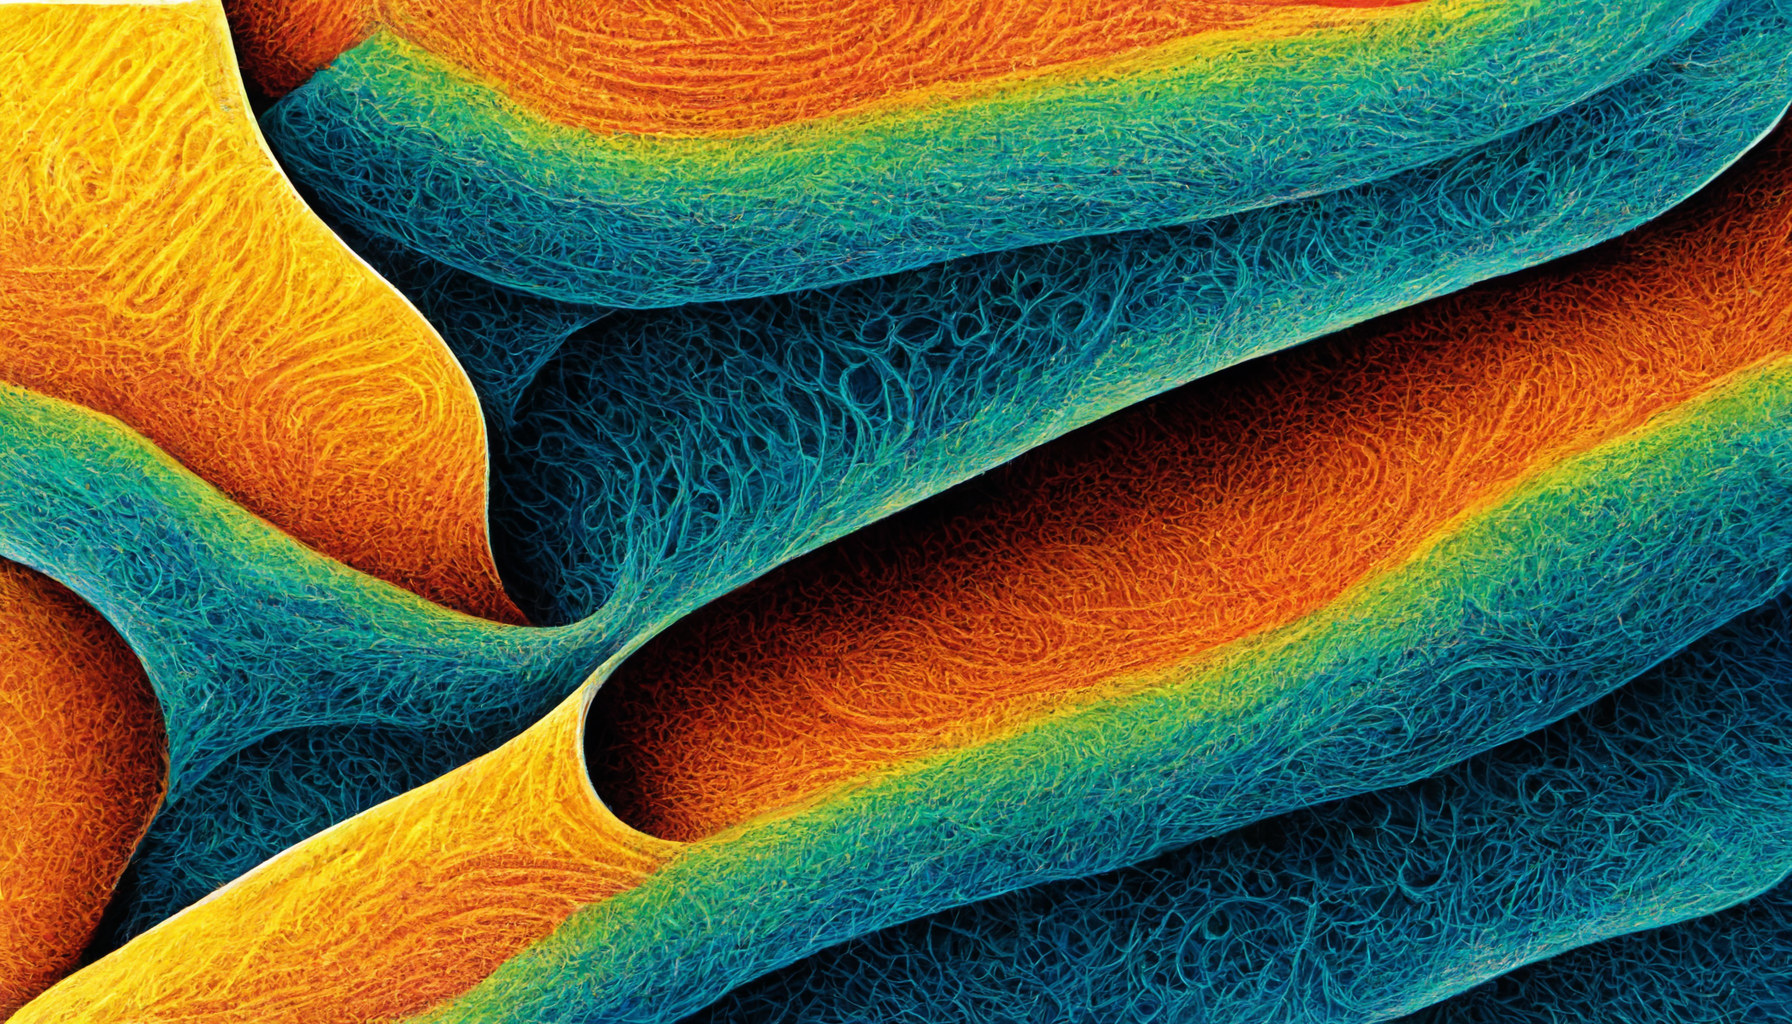
\includegraphics[width=\textwidth]{image_8}
        \end{minipage}%
        \begin{minipage}[]{0.14\textwidth}
            \centering
            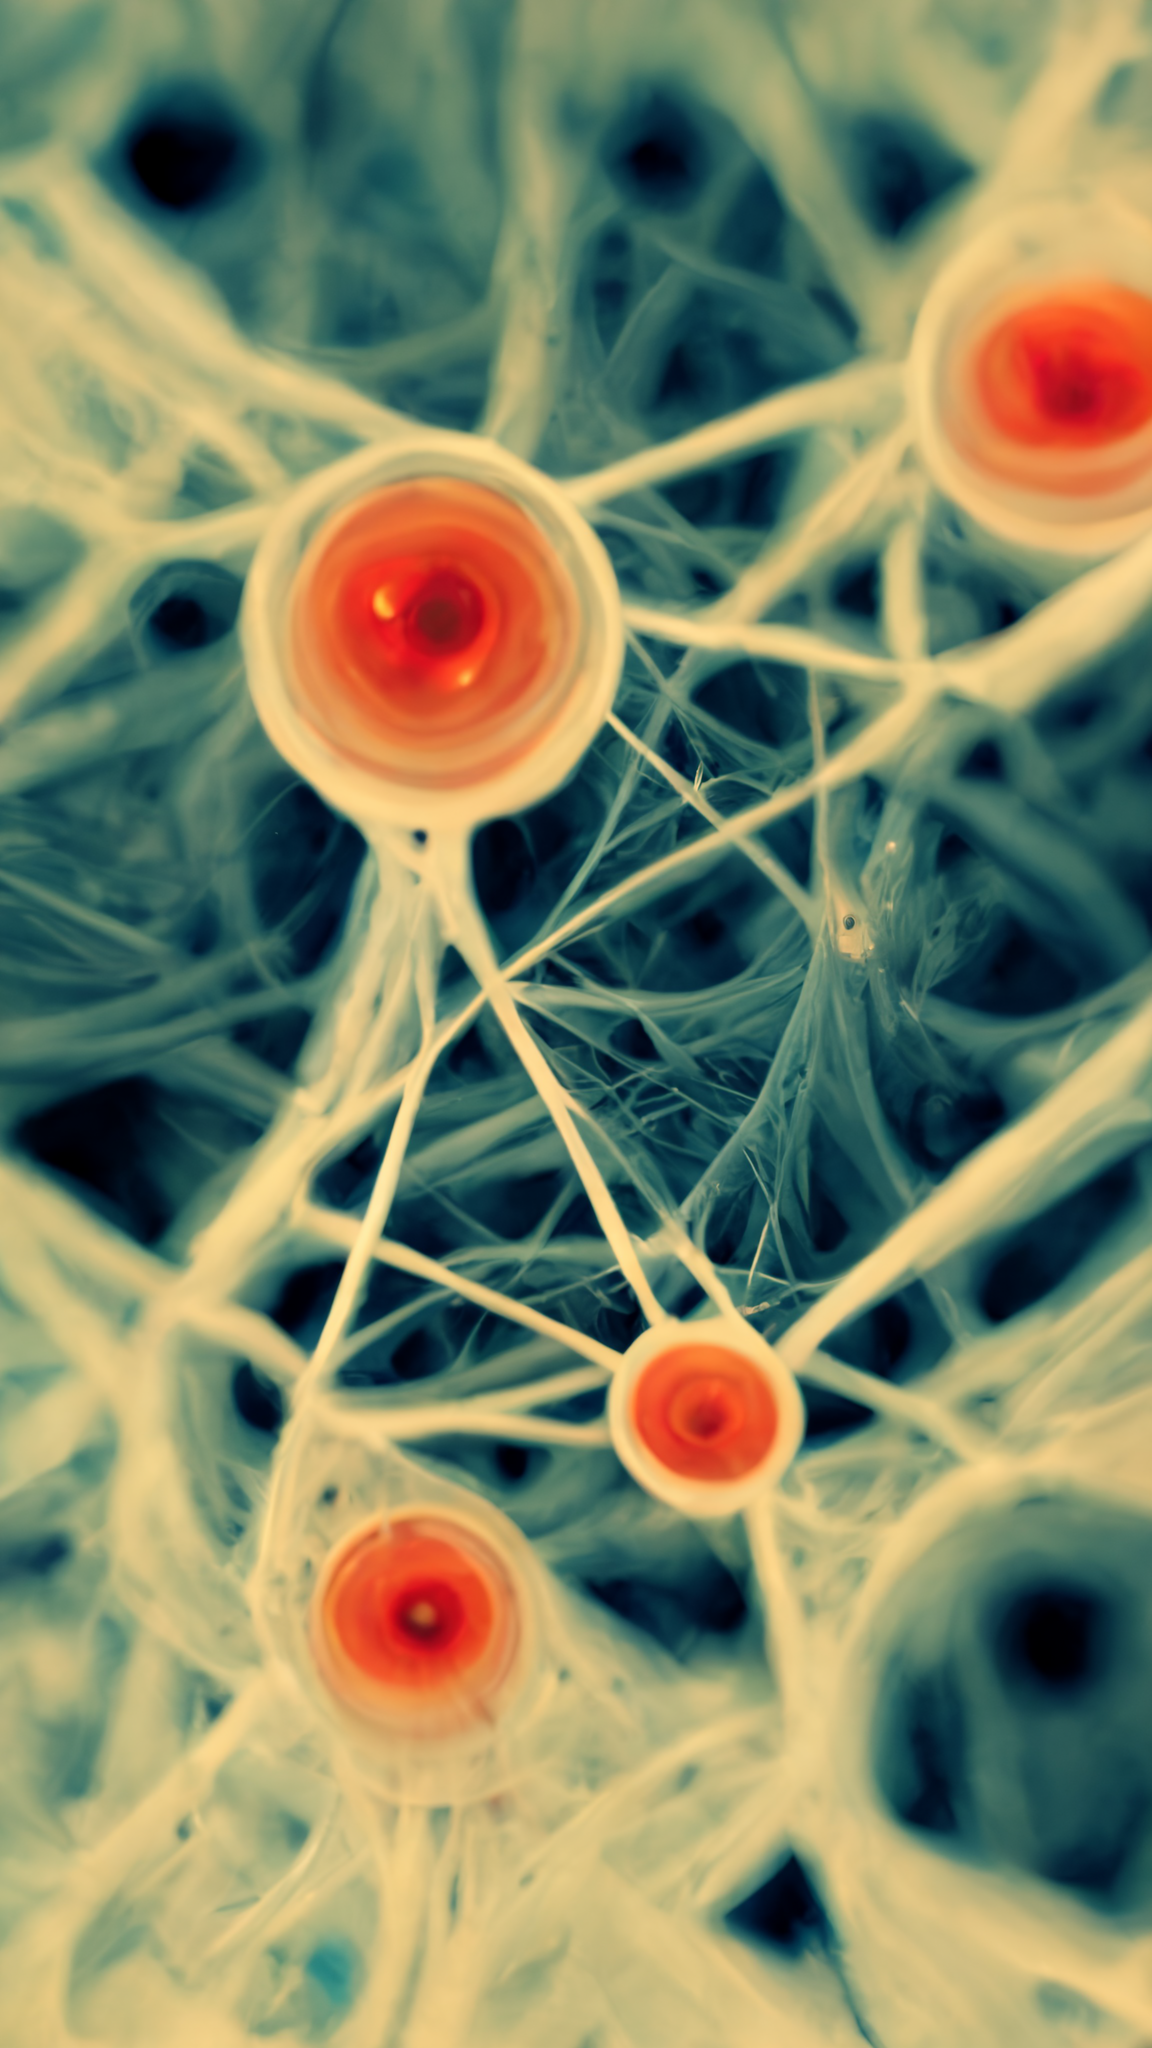
\includegraphics[width=\textwidth]{image_2}
        \end{minipage}

    }

    \block{BibTeX}{%
        As it is \LaTeX, you can use BibTeX to manage your references. Here is an example of a citation~\cite{2015MNRAS.453.4384H}. You can also use BibTeX to manage the references in the bibliography. Here is a long list: \cite{2014PhRvD..89f3505H, 2015MNRAS.450L..61H, 2015MNRAS.453.4384H, 2016A&A...594A...1P, 2016A&A...594A..20P, 2018A&A...619A..94P, 2018BayAn..13..873H, 2018JCAP...04..016F, 2018JCAP...04..017D, 2018JCAP...04..018C, 2018JCAP...04..019M, 2018JCAP...04..020D, 2018JCAP...04..021B, 2018JCAP...04..022N, 2018JCAP...04..023R, 2018JOSS....3..849H}. You can see these appear in the references section.
    }
    \block{Printing your poster}{
You can print your poster same day (although don't leave it this late!) at the University Print Shop. I recommend a0, portrait, lightweight cloth (which can be gently folded in a suitcase)
        \href{https://www.pdn.cam.ac.uk/other-pages/avmg/posters}{www.pdn.cam.ac.uk/other-pages/avmg/posters}
    }





    \column{0.5}

    \block{Other available commands}{
        \begin{minipage}{0.19\textwidth}
            \innerblock{Inner block 1}{%
                \lipsum[2]
            }
        \end{minipage}\hfill
        \begin{minipage}{0.25\textwidth}
            \innerblock{Inner block 2}{%
                \lipsum[3]
            }
        \end{minipage}\\
        \vspace{1em}

        \coloredbox{\lipsum[3]}

    }

    \block{Gallery}{%
        \centering
            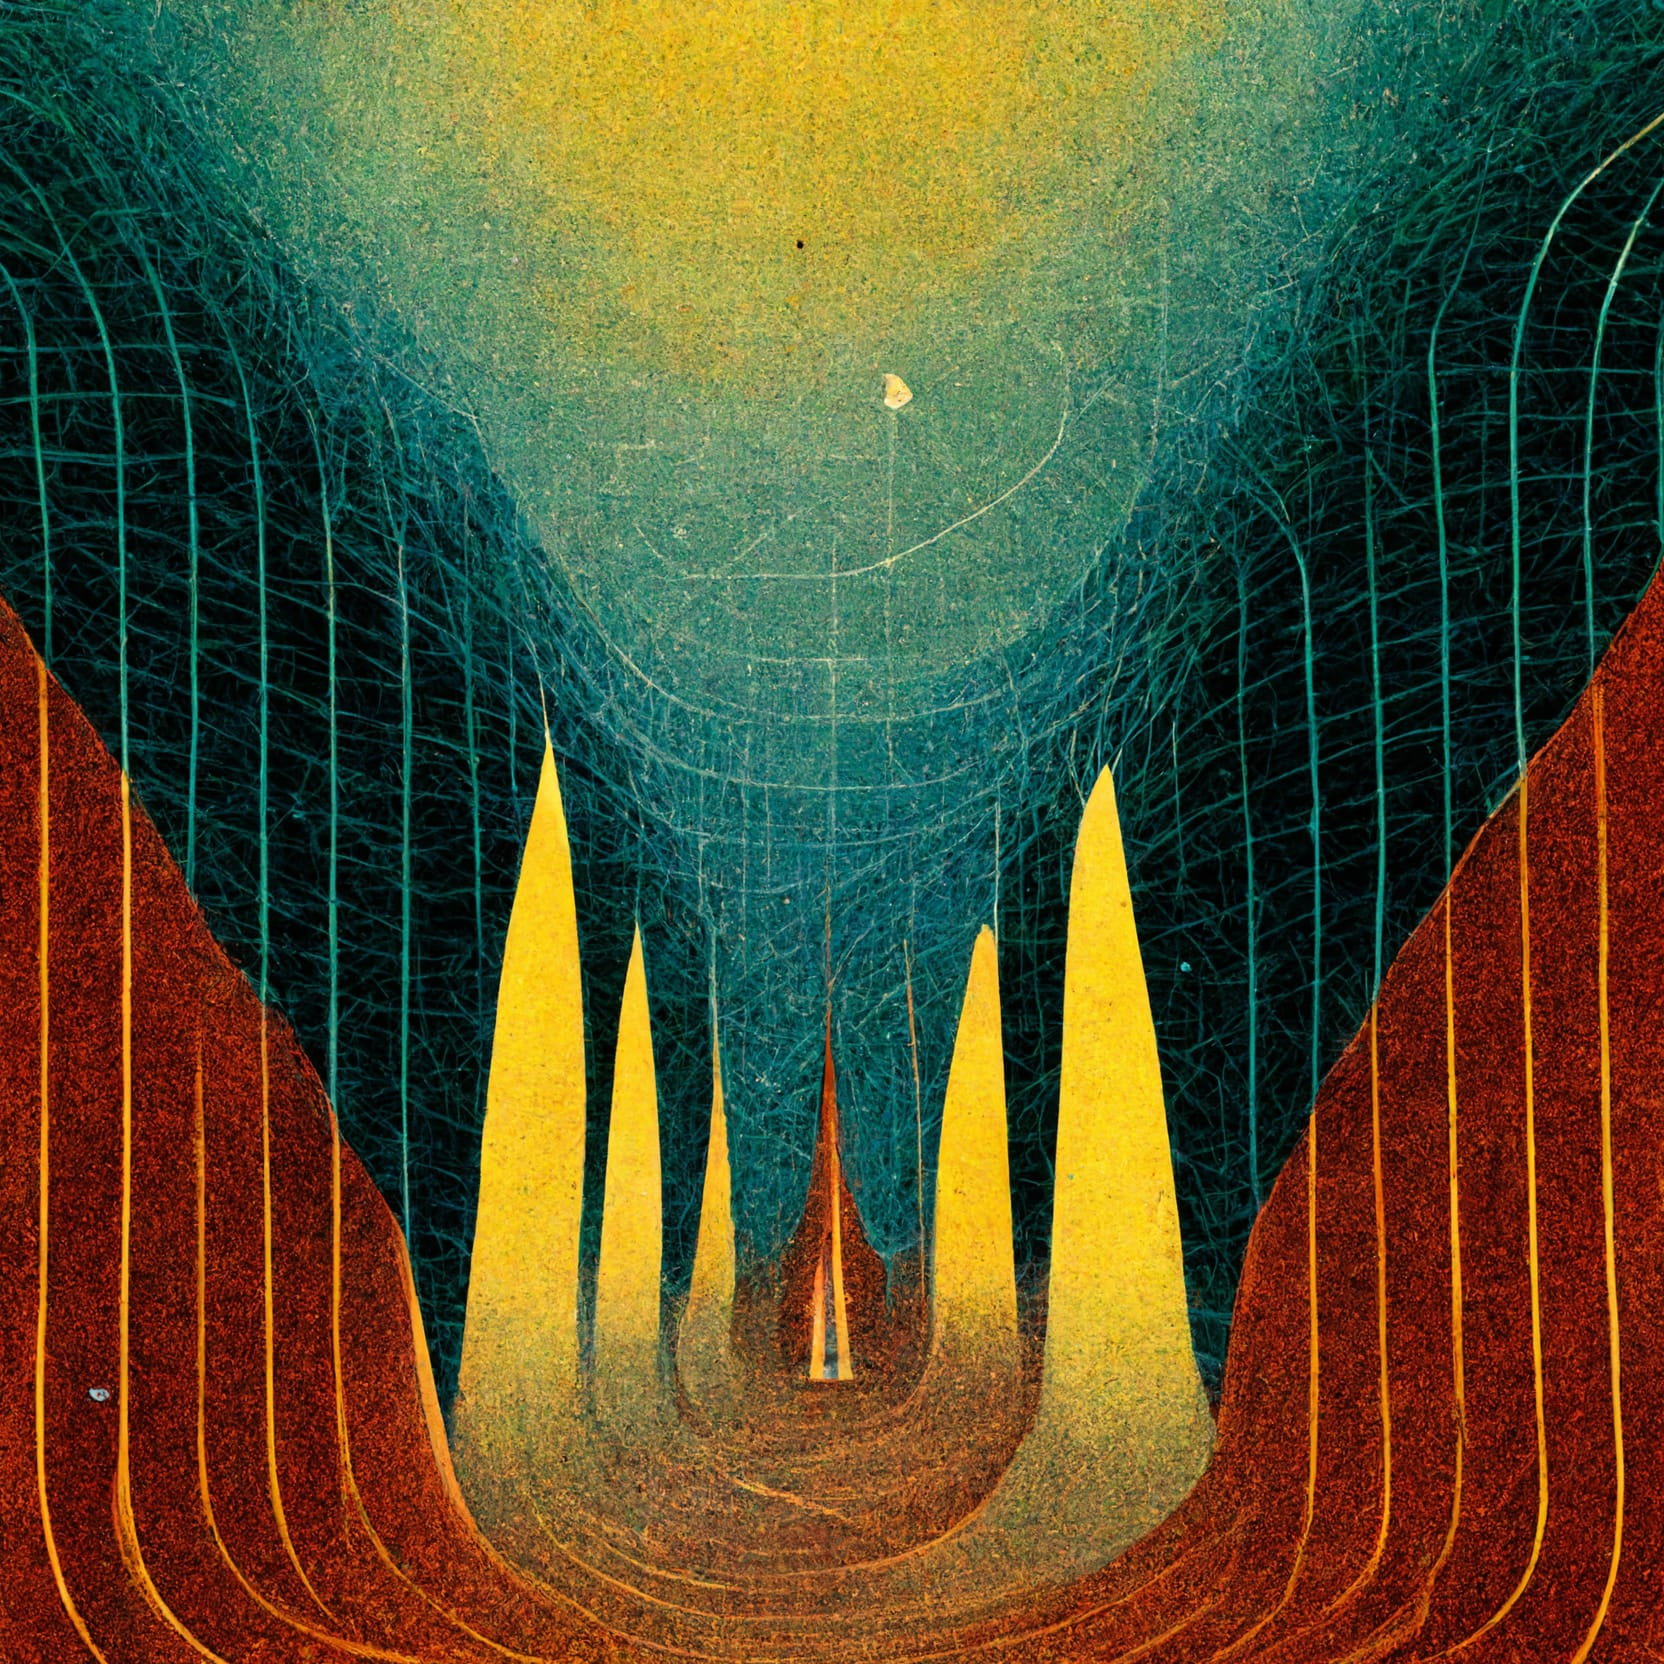
\includegraphics[height=0.1\textwidth]{image_9}%
            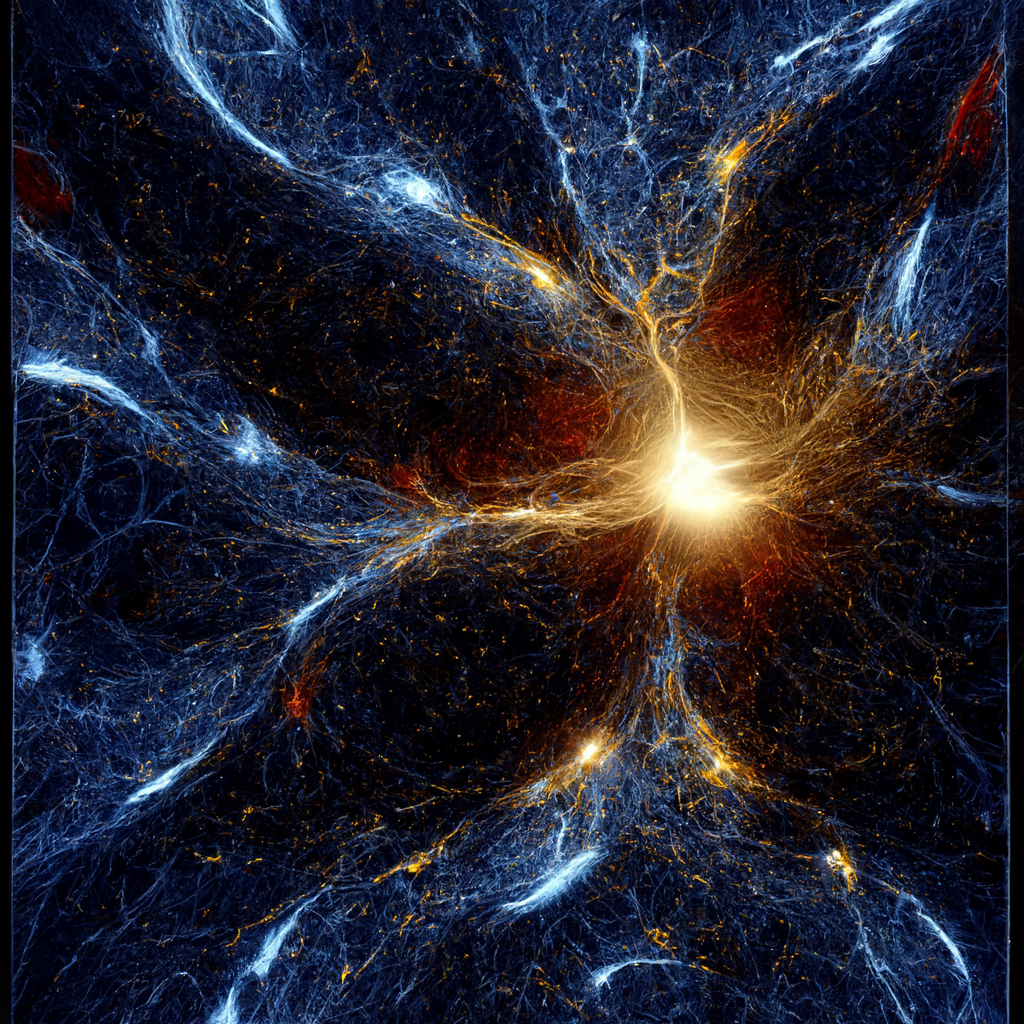
\includegraphics[height=0.1\textwidth]{image_17}%
            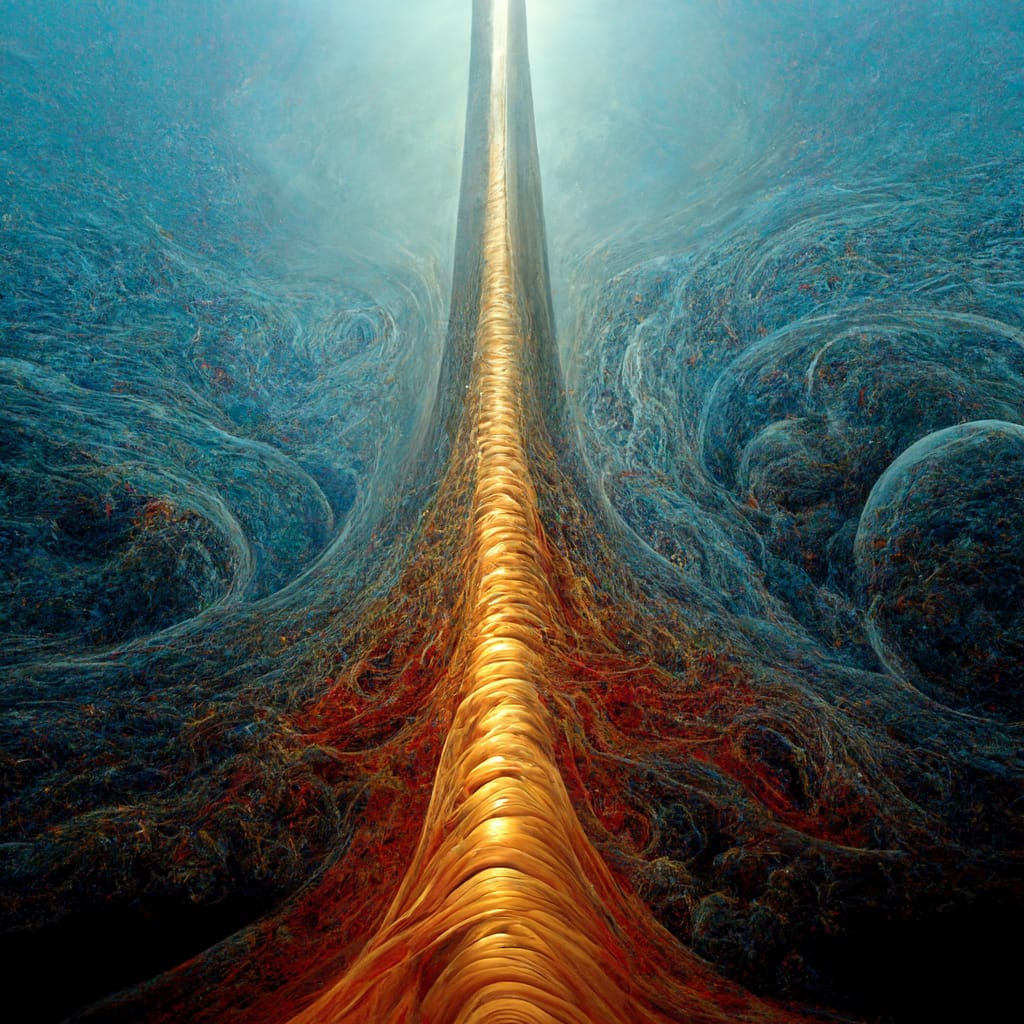
\includegraphics[height=0.1\textwidth]{image_12}%
            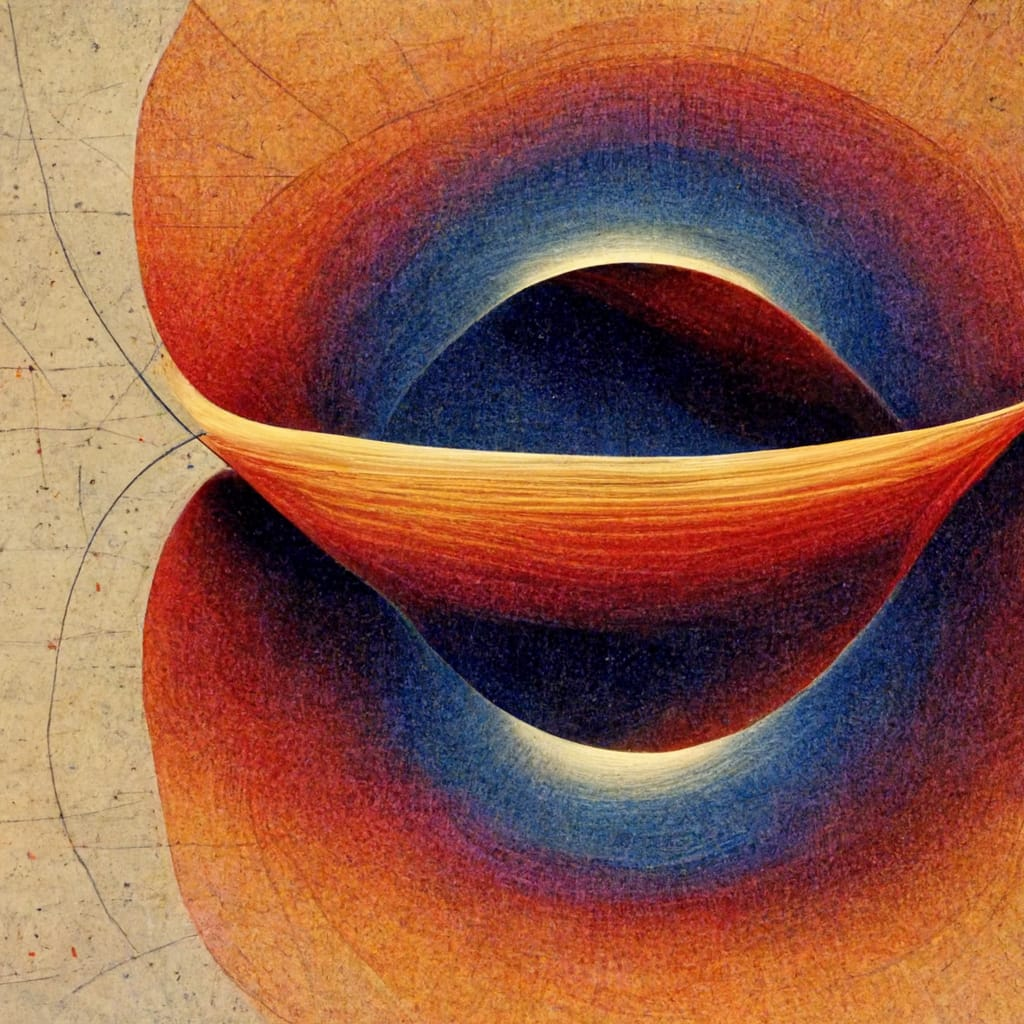
\includegraphics[height=0.1\textwidth]{image_11}\\
            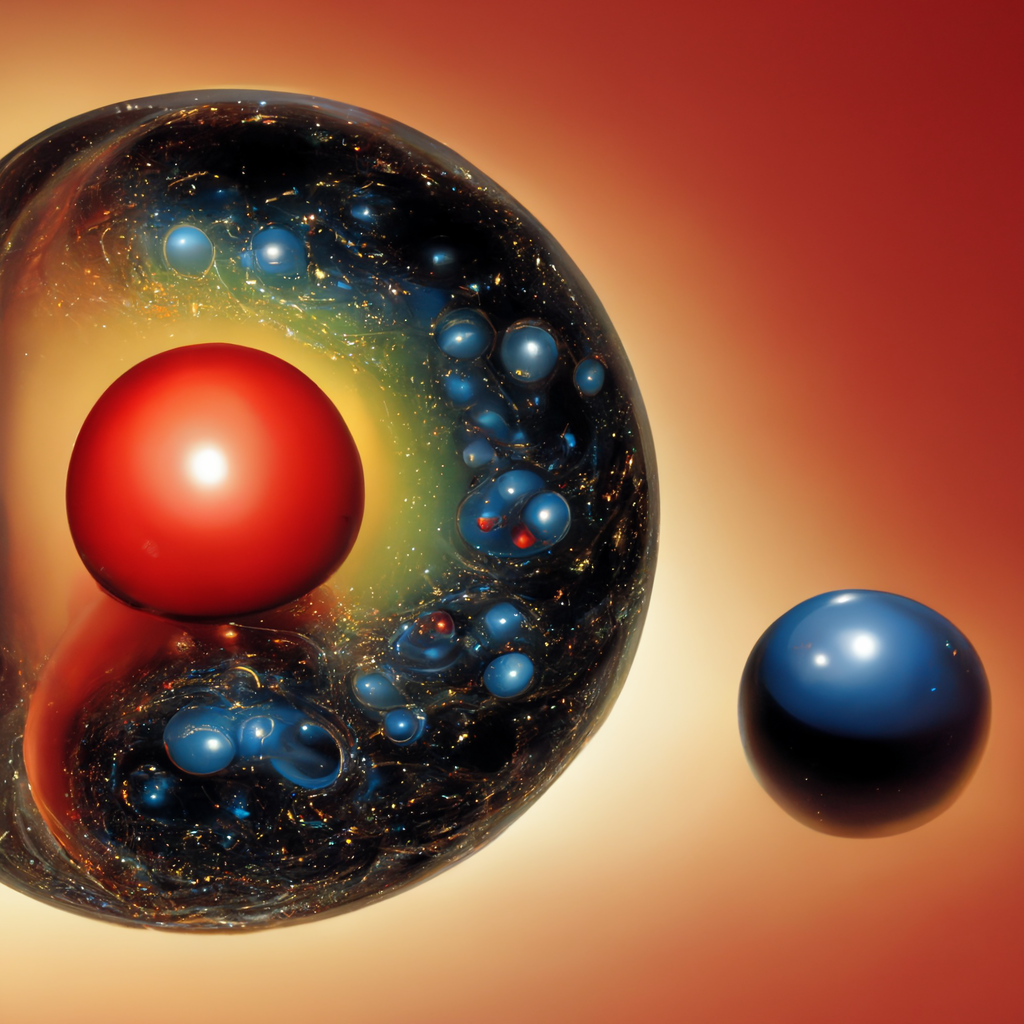
\includegraphics[height=0.1\textwidth]{image_14}%
            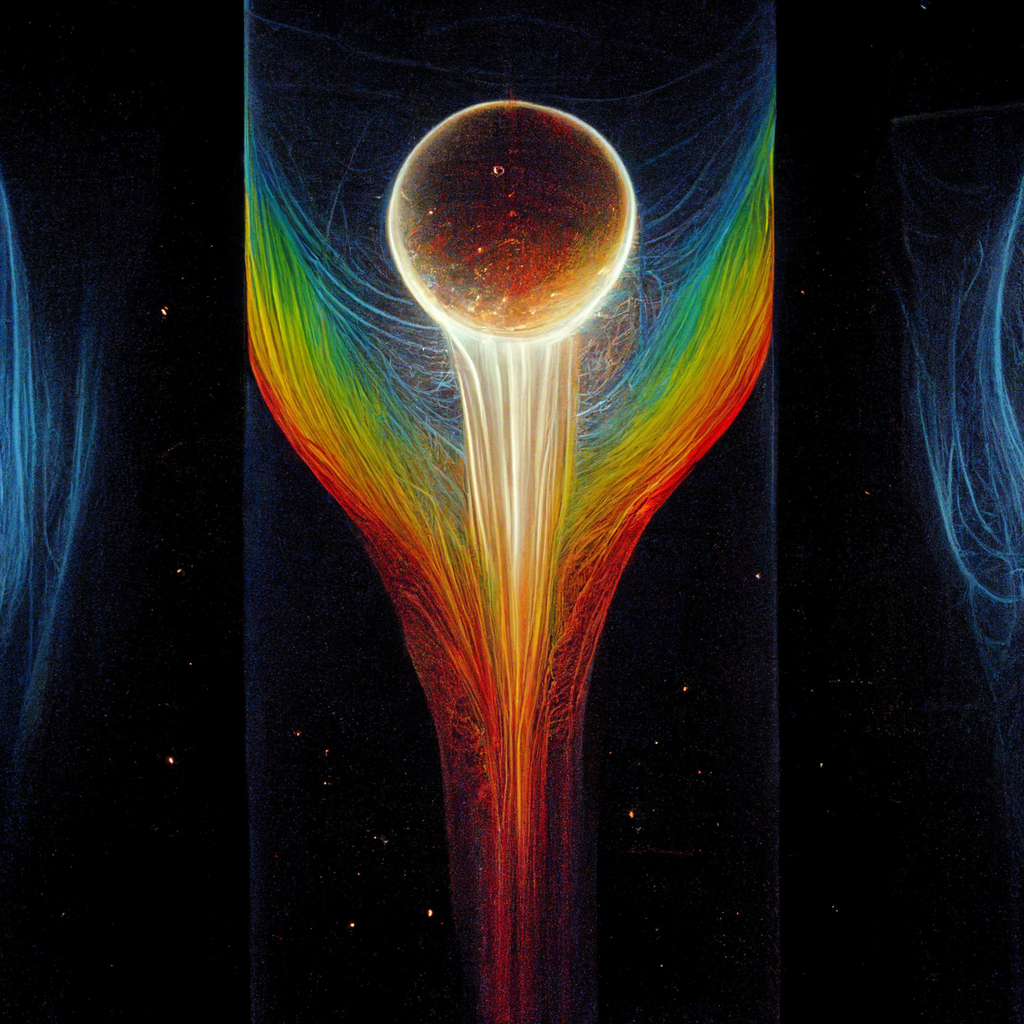
\includegraphics[height=0.1\textwidth]{image_15}%
            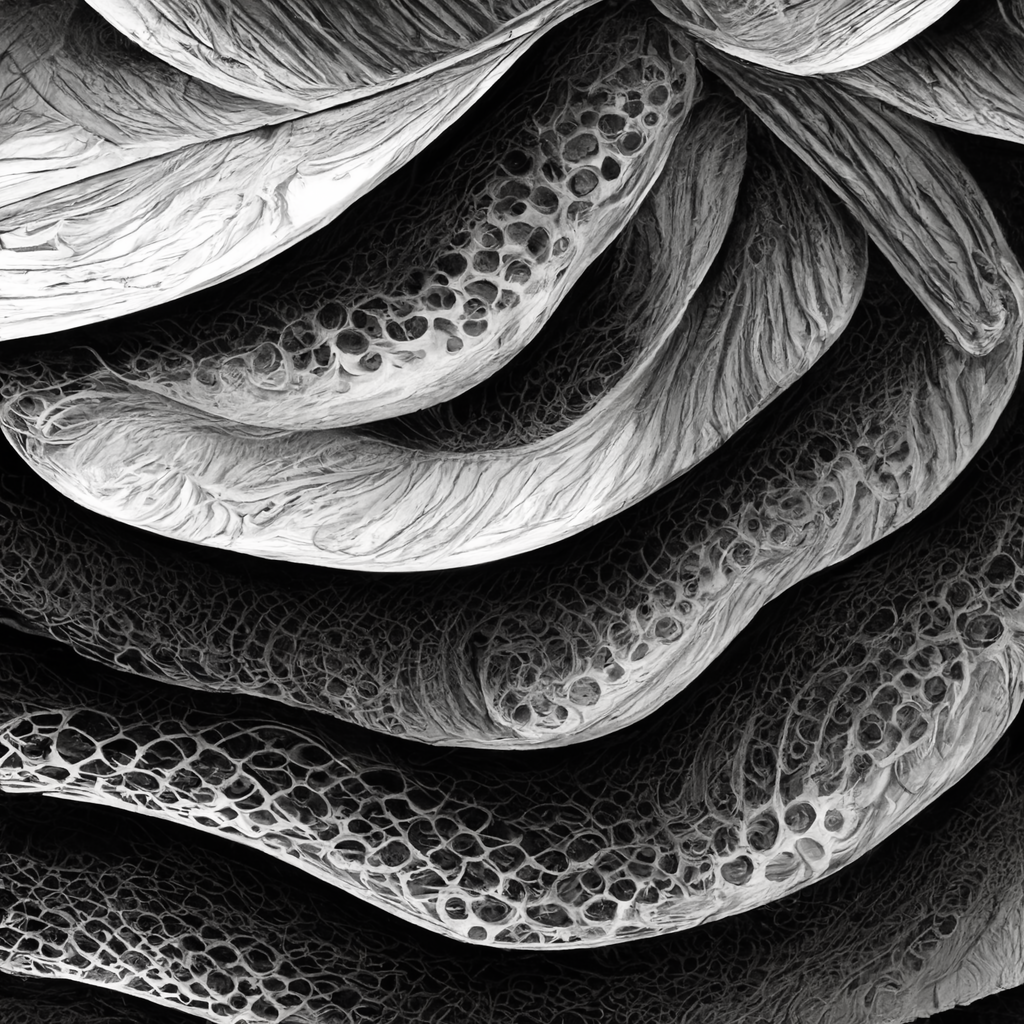
\includegraphics[height=0.1\textwidth]{image_16}%
            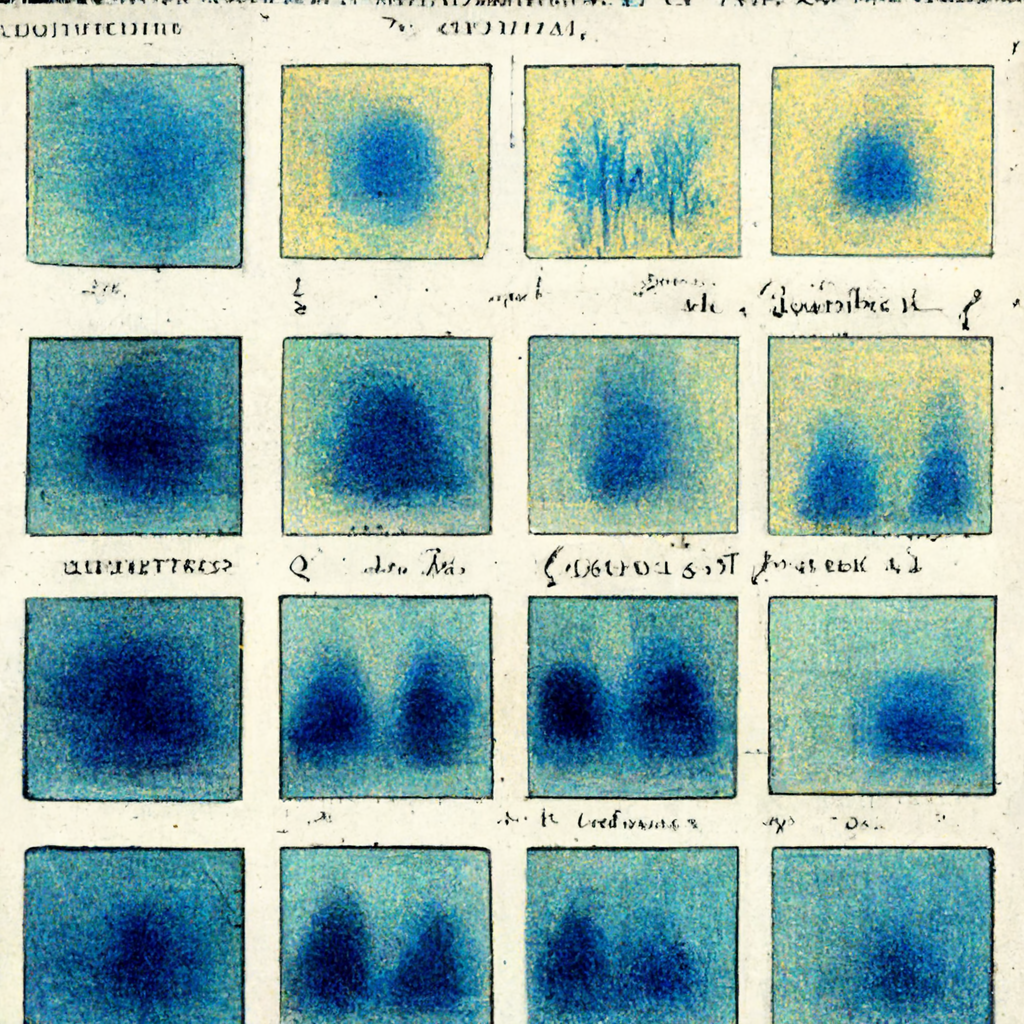
\includegraphics[height=0.1\textwidth]{image_18}%
        %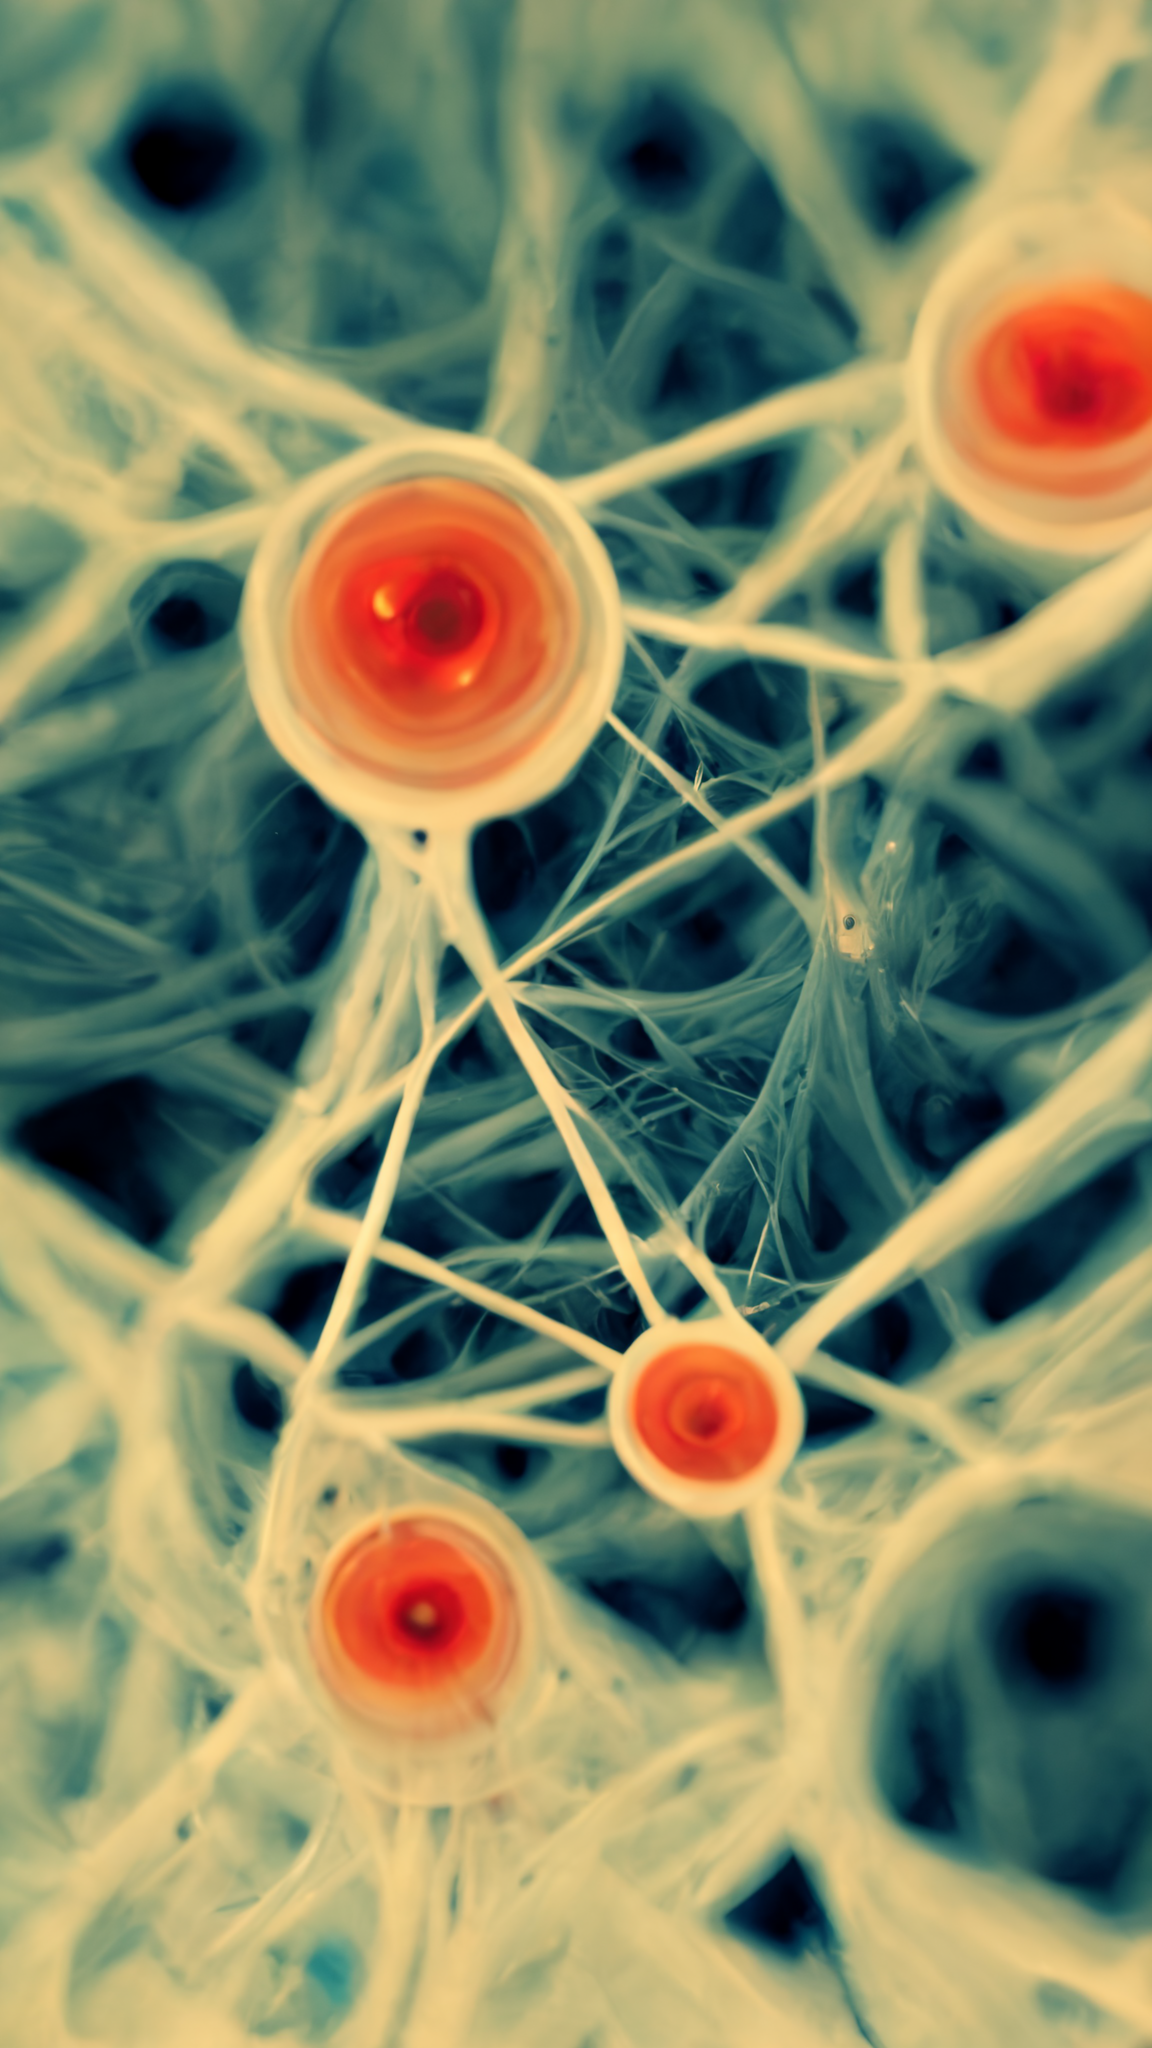
\includegraphics[height=0.095\textwidth]{image_2}%
        %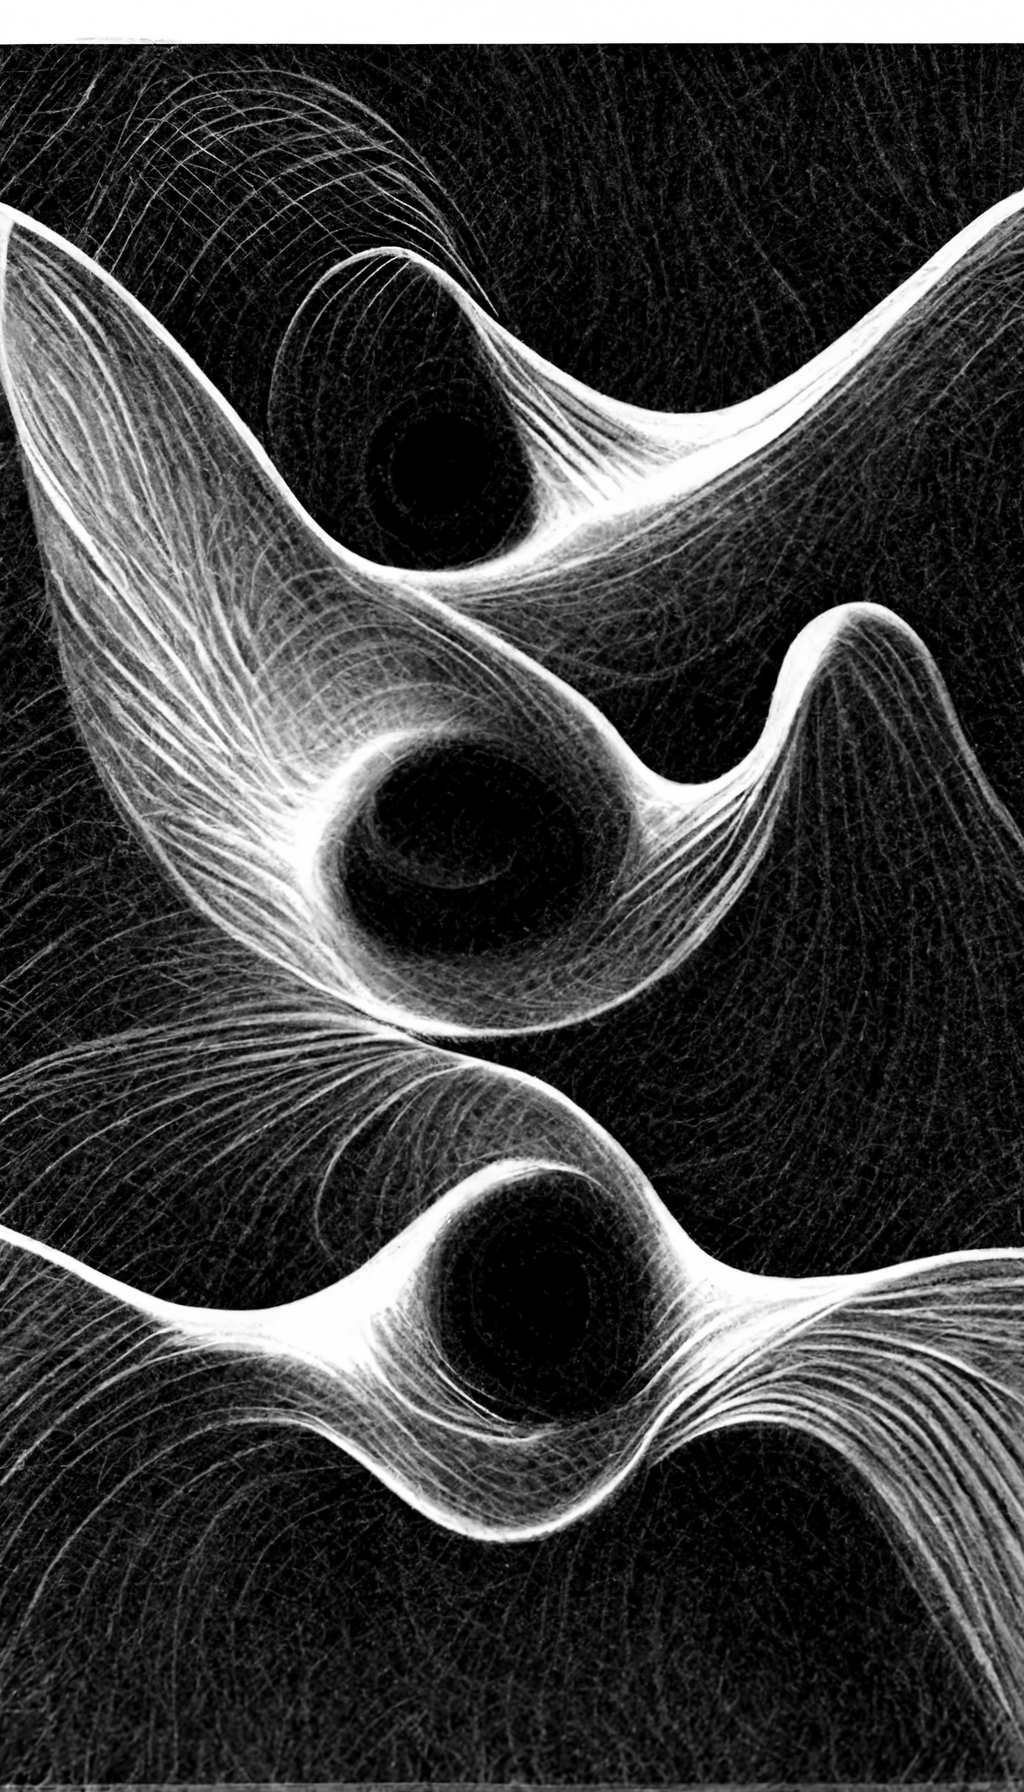
\includegraphics[height=0.095\textwidth]{image_3}%
        %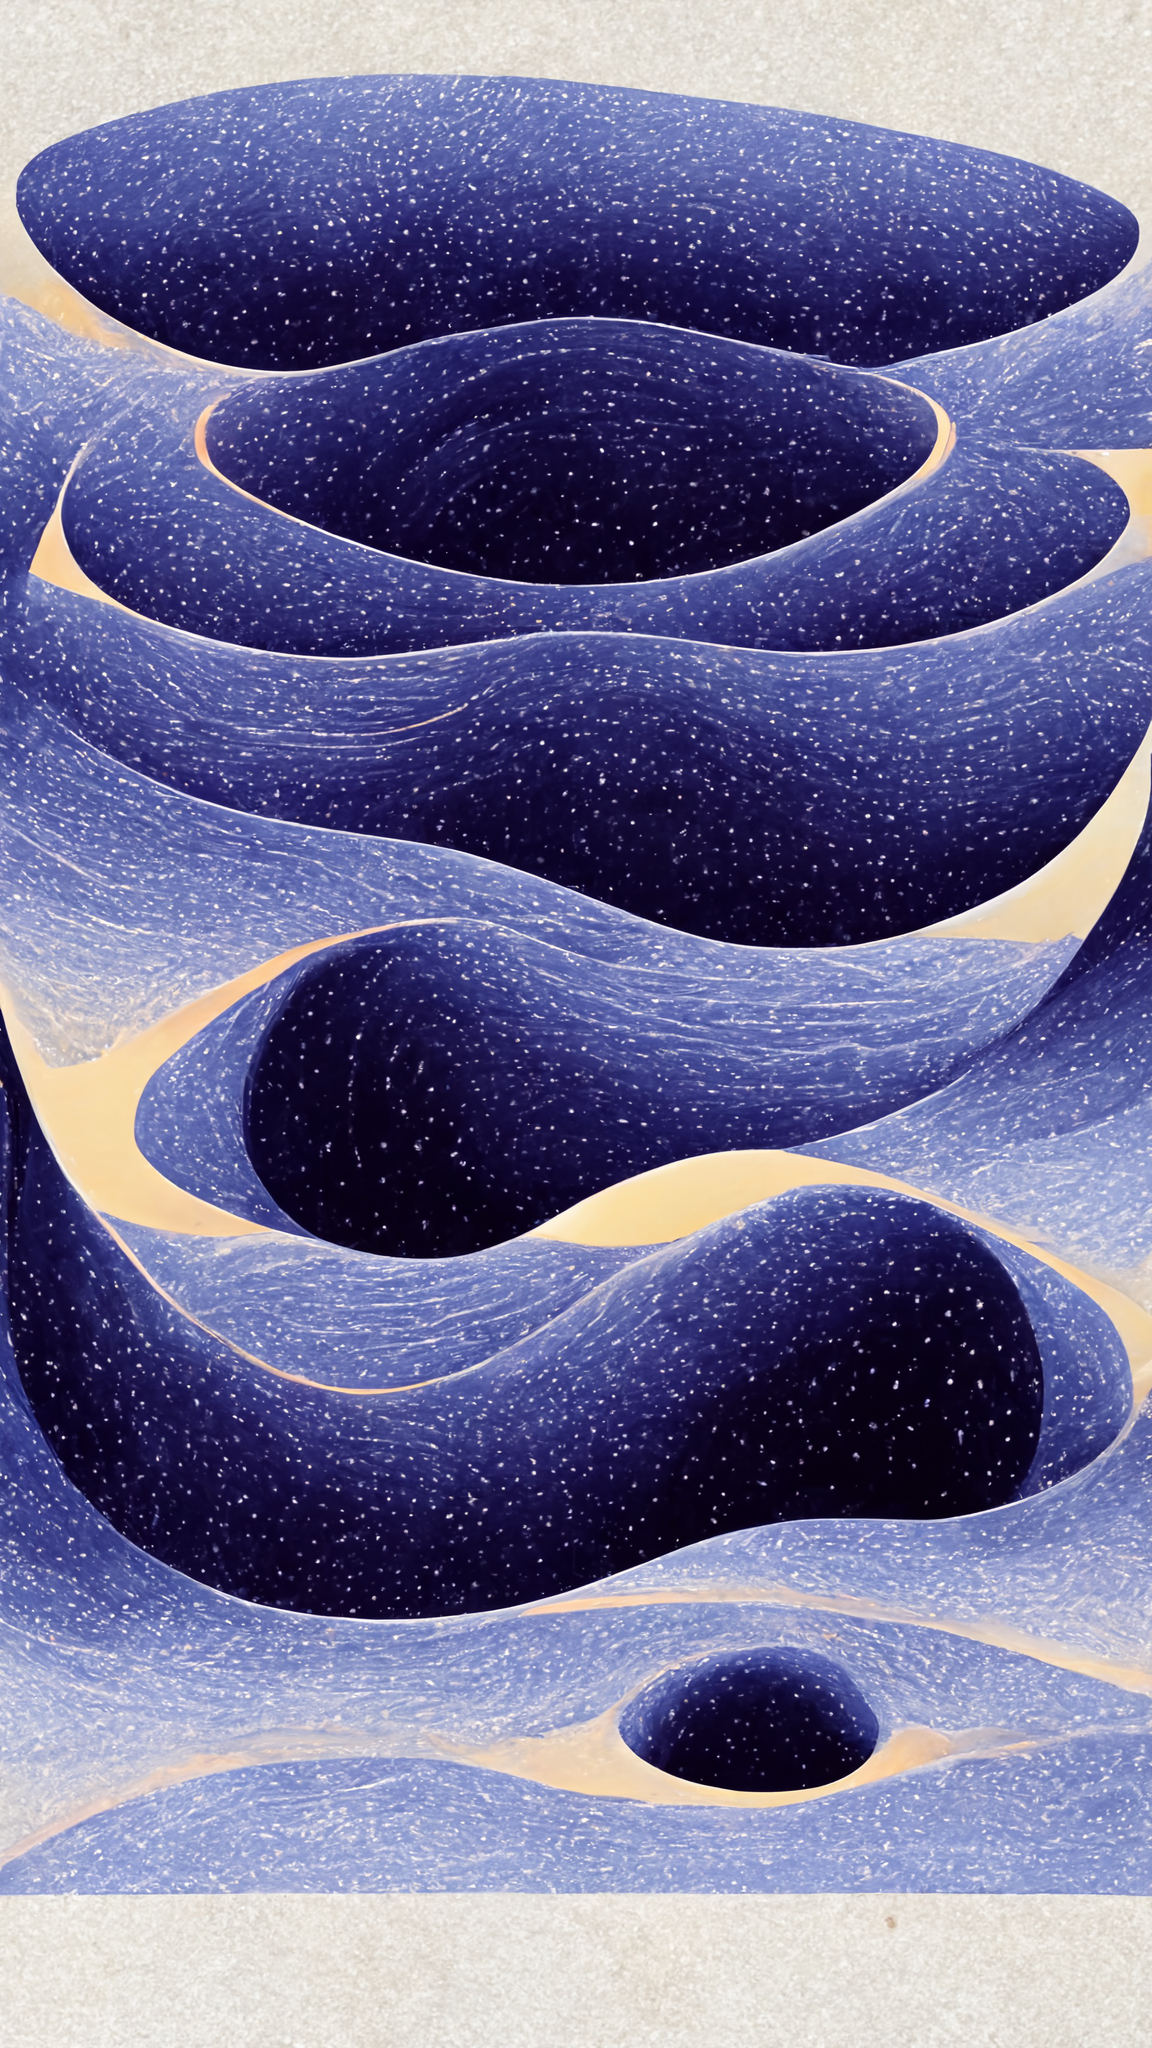
\includegraphics[height=0.095\textwidth]{image_4}%
        %\includegraphics[height=0.095\textwidth]{image_6}
        %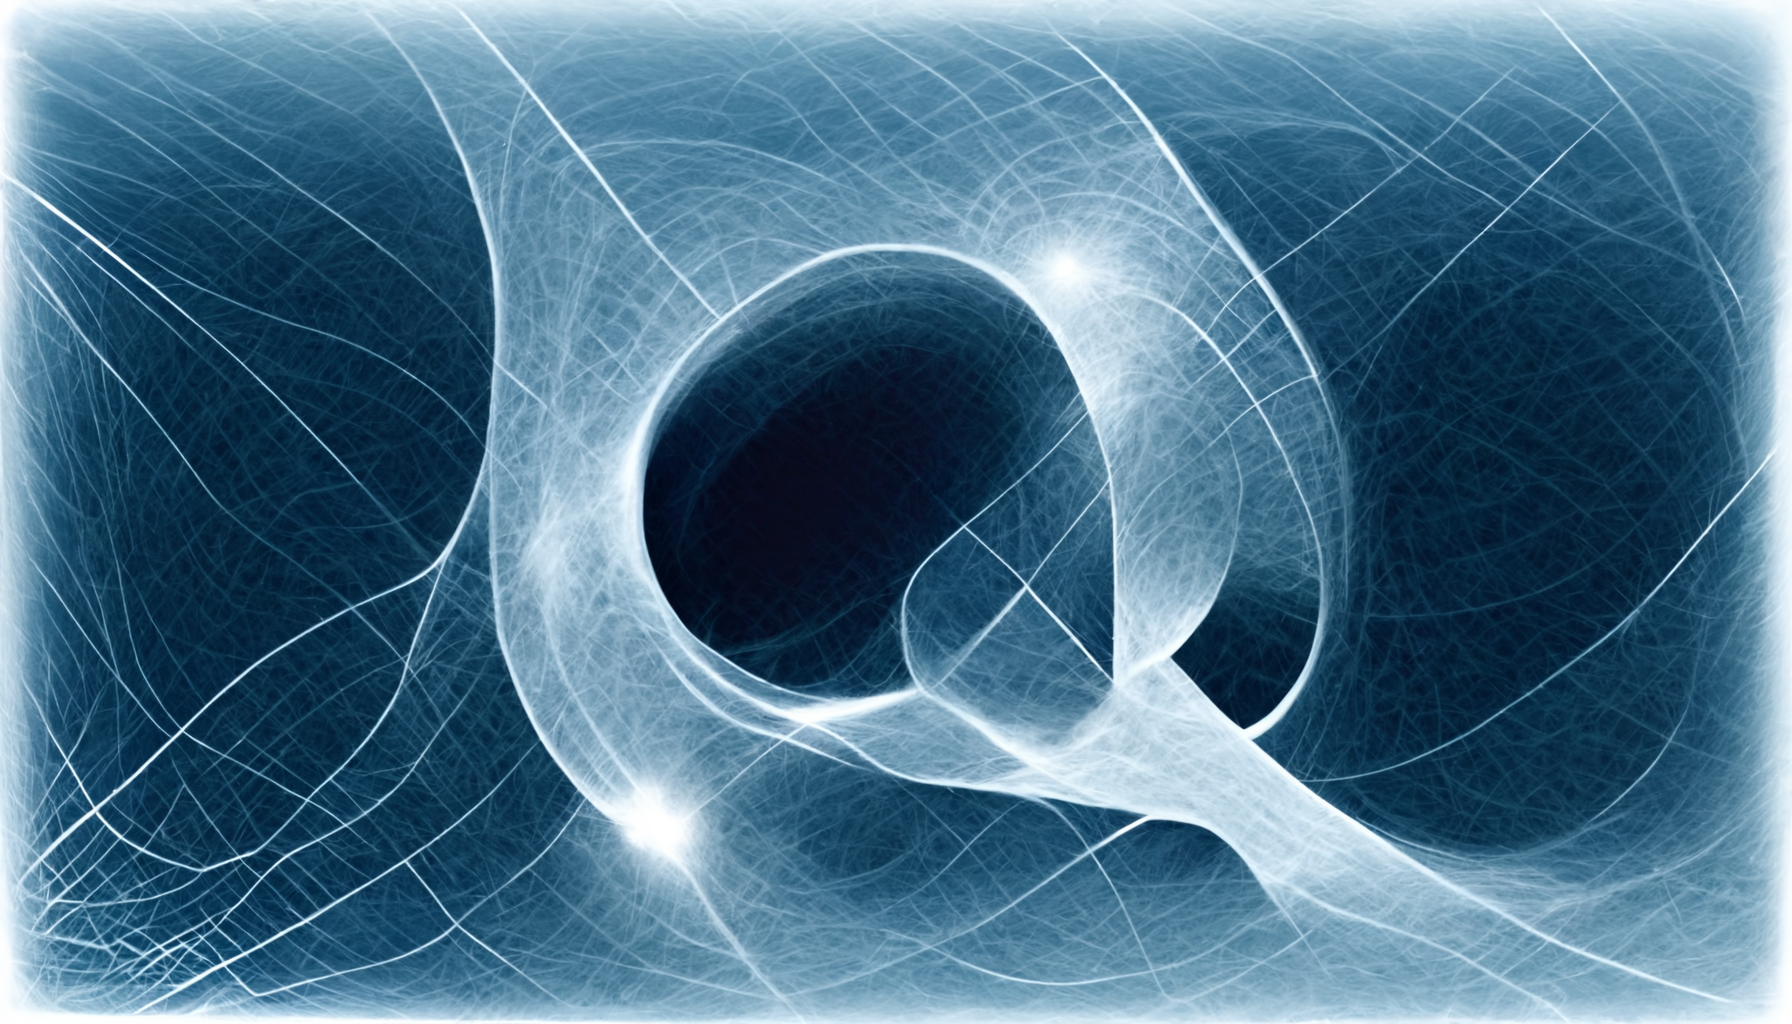
\includegraphics[height=0.095\textwidth]{image_10}
        %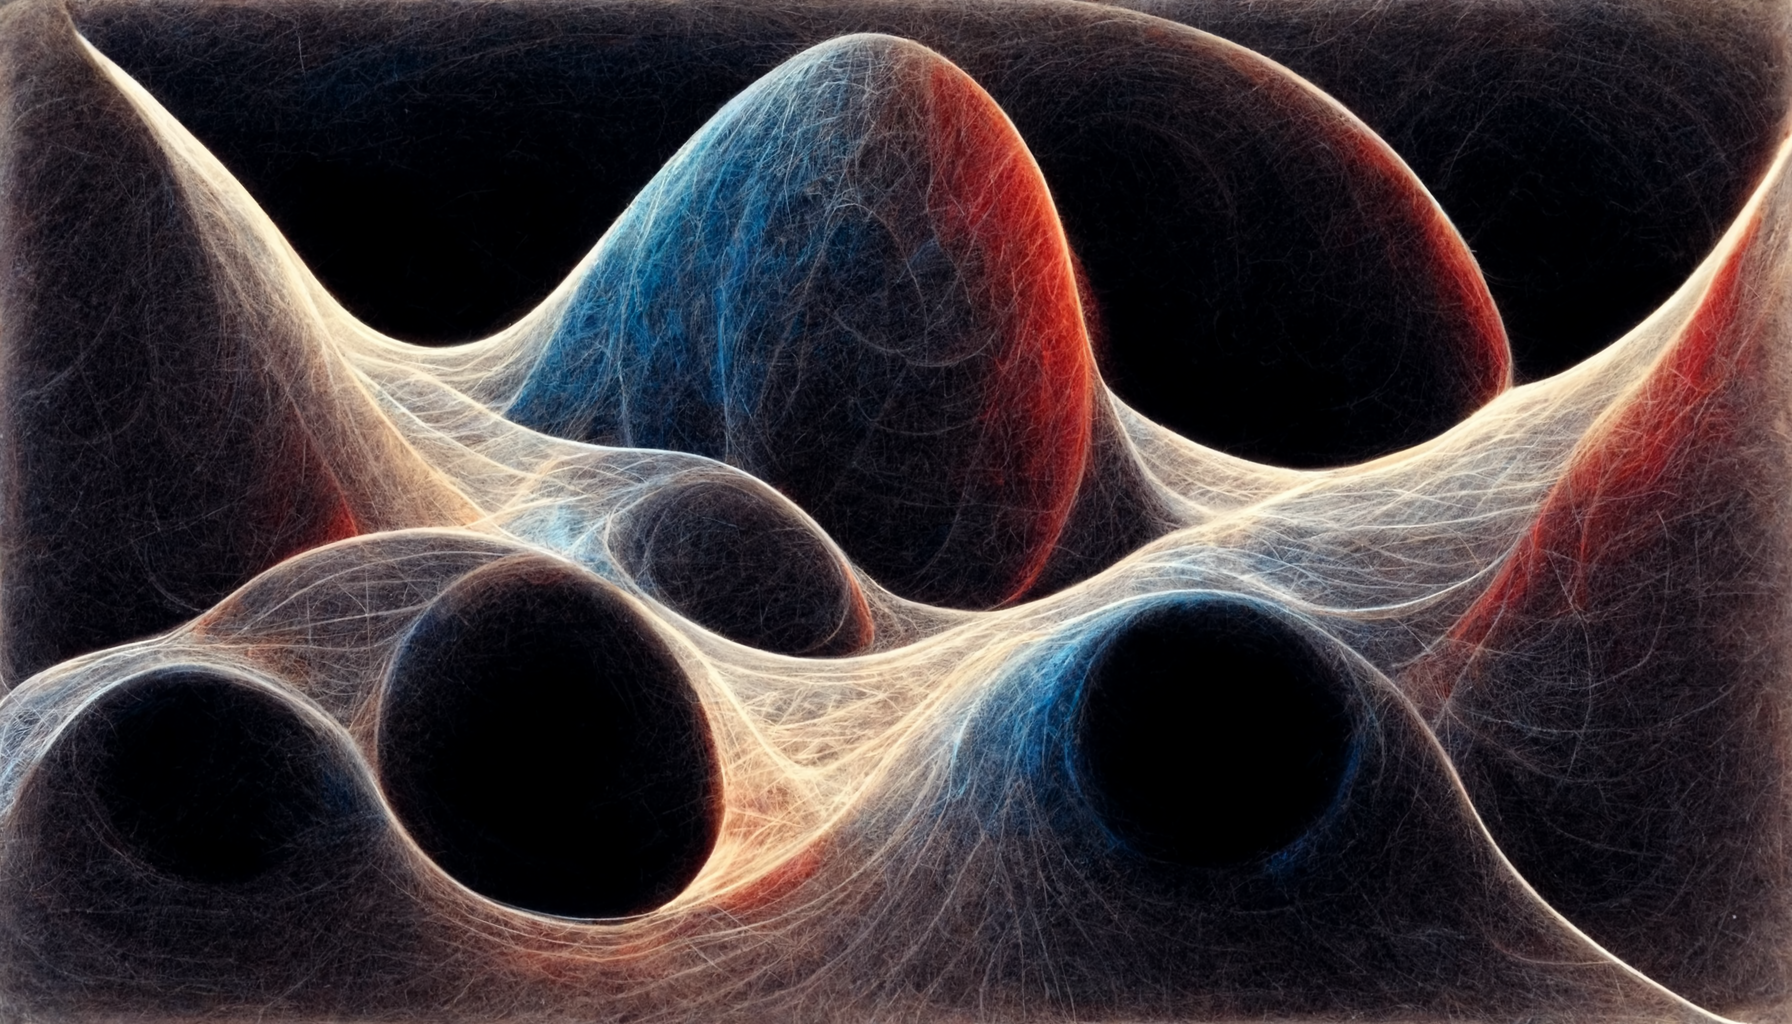
\includegraphics[height=0.095\textwidth]{image_13}
    }

    \block{Concluding box}{%
        \lipsum[4]
    }

    \renewcommand{\section}[2]{}%
    \block{References}{%
        \begin{minipage}[b]{0.35\textwidth}
            \bibliographystyle{unsrt}
            \tiny
            \bibliography{template_poster}
        \end{minipage}%
        
\includegraphics[width=0.1\textwidth]{QR.png}
    }

    \note[targetoffsetx=0.18\textwidth,targetoffsety=0.04\textwidth, connection,angle=135,radius=0.08\textwidth]{zenodo repository with thesource code and pdf for this poster.}
\end{columns}
\end{document}
